%%%%%%%%%%%%%%%%%%%%%%%%%%%%%
\section{Calibration strategy}
\label{sec:calibration}
%%%%%%%%%%%%%%%%%%%%%%%%%%%%
For the calibration procedure described in this note, dimuons from the decay of
Z bosons were used. 
The invariant mass spectrum of the dimuons 
was modeled as the sum of a signal obtained from a NNLO
calculation~\cite{Dittmaier:2009cr}, adapted to kinematic cuts close to
those used in the selection of reconstructed muons, and an
exponentially falling background. The decay constants of the
exponential were determined separetely in 16 bins, each one corresponding to each 
muon's pseudorapidity falling in one of the following ranges: [-2.4,-0.8], [-0.8,0], 
[0,0.8], [0.8,2.4]. A representation of the signal model as a function of the dimuon mass 
and the dimuon resolution is shown in Figure \ref{fig:lineshape}.\\
The datasets used, corresponding to both collision data and simulated events reconstructed in the CMS 
detector, are listed in table~\ref{tab:datasets}.
%%%%%%%
\begin{table}[hbH]
\label{tab:datasets}
\begin{center}
\caption{Datasets corresponding to the different samples of data and
  simulated events used for the study of the muon momentum scale at 
  center of mass energy of $\sqrt{s}$=7 TeV and $\sqrt{s}$=8 TeV. ``Label'' is 
  how the samples are indicated later in Table~\ref{tab:scale_parameters}.\label{tab:datasets}}
\resizebox{\textwidth}{!}{\begin{tabular}{|llll|}
\hline
$\sqrt{s}$ & Type & Dataset name & Label \\
\hline
7 TeV & data & /DoubleMu/Run2011A-08Nov2011-v1,           &2011\_DATA\_44X      \\
                 & data & /DoubleMu/Run2011B-19Nov2011-v1 &                     \\
 & Monte Carlo & /DYJetsToLL\_TuneZ2\_M-50\_7TeV-madgraph-tauola/Fall11-PU\_S6\_START44\_V9B-v1                                    &2011\_MC\_44X        \\
\hline
8 TeV & data & /DoubleMu/Run2012A-22Jan2013-v1,     &2012ABC\_DATA\_ReReco\\
                & data & /DoubleMuParked/Run2012B-22Jan2013-v1,    & \\ 
                & data & /DoubleMuParked/Run2012C-22Jan2013-v1     & \\
 & data & /DoubleMuParked/Run2012D-22Jan2013-v1                                                                             &2012D\_DATA\_ReReco\_53X  \\
 & Monte Carlo & /DYJetsToLL\_M-50\_TuneZ2Star\_8TeV-madgraph-tarball/DR53X-PU\_S10\_START53\_V7A-v1                               &2012\_MC\_ReReco\_53X     \\
 & Monte Carlo & /Upsilon1SToMuMu\_2MuPtEtaFilter\_tuneD6T\_8TeV-pythia6-evtgen/Summer12\_DR53X-PU\_S10\_START53\_V7A-v1           & \\
 & Monte Carlo & /JPsiToMuMu\_2MuPtEtaFilter\_tuneD6T\_8TeV-pythia6-evtgen/Summer12\_DR53X-PU\_S10\_START53\_V7A-v2                 & \\
\hline
\end{tabular}}
\end{center}
\end{table}

%%%%%

Corrections were derived for the so-called {\it global
  muons}~\cite{Chatrchyan:2013sba} using as $p_T$ the one measured by
the inner silicon tracker. To ensure low contamination, reconstructed
muons were further selected according to the criteria detailed in
table~\ref{tab:muon_selection}

\begin{table}[hbH]
\begin{center}
\caption{Selection of reconstructed muons.\label{tab:muon_selection}}
\begin{tabular}{|l|ll|}
\hline
$\sqrt{s}$=7 TeV & Kinematics and topology:& $p_T>$ 20 GeV $|\eta|<$2.4 $d_{xy}<$ 0.2 cm \\
                 & Isolation: & $I^{rel}_{comb}<0.15 p_T$ \\
                 & Track quality: & $N_{hits}$  tracker $>10$ \\ && $N_{hits}$ pixel $>0$ \\&& $N_{hits}$ muons $>0$ \\&&  $\chi^2/ndof < 10$ \\
& & $N_{mu-stations}$ matched $>1$  \\
\hline
$\sqrt{s}$=8 TeV & Kinematics and topology:& $p_T>$ 20 GeV $|\eta|<$2.4 $d_{xy}<$ 0.2 cm $d_{z}<$5 cm \\
& Isolation: & $I^{PF}_{boh?}<0.12 p_T$ \\
& Track quality: & $N_{tk-layers}$ with measurements $>5$  \\ && $N_{hits}$ pixel $>0$\\
& & $N_{mu-stations}$ matched $>1$  \\
\hline
\end{tabular}
\end{center}
\end{table}

%%%%%
\begin{figure}[hbtp]  
\begin{center}
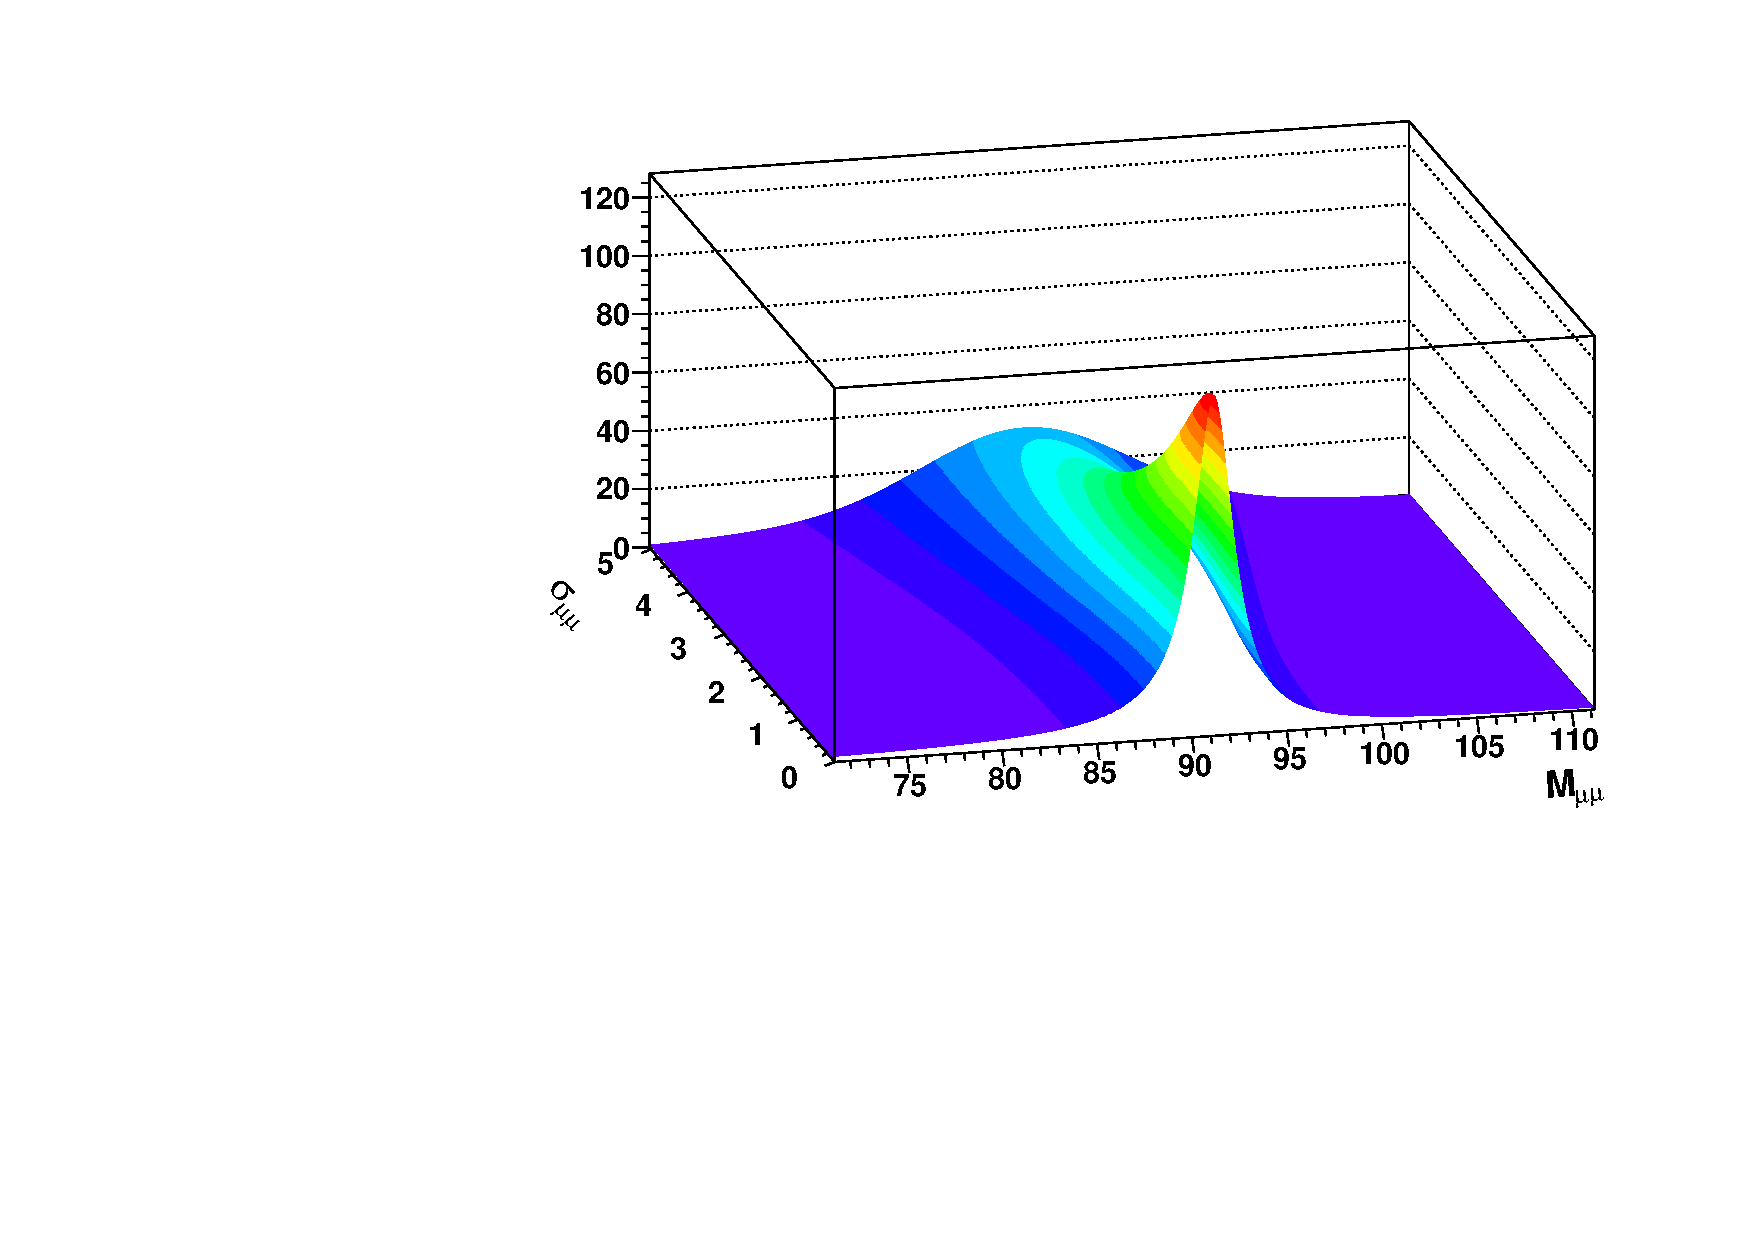
\includegraphics[width=0.7\textwidth]{figures/Lineshape_SURF2}
 \hspace{1cm} 
   \caption{Signal model used in the MuScleFit likelihood, as a function of the dimuon mass resolution
   \label{fig:lineshape}}
 \end{center}
\end{figure} 


% $\eta(\mu^+)$ $\eta(\mu^-)$ 
%\FIXME description of MF strategy (scale no $p_0$, resolution, scale $p_0$ only, resolution) /ingredients\\
%\FIXME quote SDittmaier
%The ansatz functions describing the scale
%corrections and the resolution entering in the construction of
%the likelihood are detailed below.
%%%%%%%%%%%%%%%%%%%%%%%%%%%%%%%%%%%%%%%%%%%%%%%%%%%%%%
\subsection{Ansatz functions for scale corrections and resolution}
%%%%%%%%%%%%%%%%%%%%%%%%%%%%%%%%%%%%%%%%%%%%%%%%%%%%%%
%To derive a reference value of the mass of the 
%The reconstructed invariant mass specturm of the dimuon was fitted
%with the Table~\ref{tab:fit_pdfs}
Figure~\ref{fig:etaphi_44X_before} (left) shows the 
mass of the Z boson extracted from the reconstructed 
invariant mass spectrum of the dimuon in bins of
($\varphi$,$\eta$) of the positive muon for the data at
$\sqrt{s}$=7~TeV.
In each bin, the reconstructed invariant mass
was fitted with the pdf described in Table~\ref{tab:fit_pdfs}: 
the fitted pole of the Breit-Wigner was taken as the mass of the boson 
while the sigma of the Crystal Ball was taken as the resolution.

%%%%%%%
\begin{table}[hbH]
\begin{center}
\caption{Probability density functions (pdf's) used to extract the mass of
  the  J/$\psi$, $\Upsilon(1S)$ and Z resonances from the spectrum of
  the dimuon invariant mass $x$.
  $CB(x)$ is the Crystal Ball pdf, $BW(x)$ is the Breit-Wigner pdf,
  ``n$^{th}$ order Bern$(x)$'' is the n$^{th}$ order Bernstein
  polynomial pdf.\label{tab:fit_pdfs}}
\begin{tabular}{|ll|c|c|c|}
\hline
Resonance & & Fit Range [GeV] & Signal pdf & Background pdf \\
\hline
J/$\psi$       & DATA & [2.9,3.3] & $CB(x,\mu,\sigma)$ & 3$^{rd}$ order Bern. pol. \\
               & MC   & [2.9,3.3] & $CB(x,\mu,\sigma)$ & 3$^{rd}$ order Bern. pol. \\
\hline
$\Upsilon(1S)$ & DATA & [8.7,11.0] &$CB_(x,\mu_1,\sigma)+CB(x,\mu_2,\sigma)$ & 4$^{th}$ order Bern. pol. \\
               &      &            &$+CB(x,\mu_3,\sigma)$ & \\
               & MC   & [8.8,10.0] & $CB_(x,\mu,\sigma)$            & 4$^{th}$ order Bern. pol. \\
\hline
Z              & DATA & [75,105] & $BW(x,\mu,\Gamma_Z) \otimes CB(x,0,\sigma)$ & $\exp(a_0+a_1x+a_2x^2)$  \\
               & MC   & [75,105] & $BW(x,\mu,\Gamma_Z) \otimes CB(x,0,\sigma)$ & $\exp(a_0+a_1x+a_2x^2)$  \\
\hline
\end{tabular}
\end{center}
\end{table}
Offsets with respect the nominal mass of the Z up to 2 GeV are observed. 
Offsets are also observed in simulated events
(Figure~\ref{fig:etaphi_44X_before} right) as the conditions of 
the detector used in the reconstruction of simulated events reproduce the
level of knowledge of the detector in the data, hereafter referred to
as {\sl realistic} conditions.
\begin{figure}[hbtp]  
\begin{center}
\includegraphics[width=0.45\textwidth]{figures/TkAl_Style/Data2011_44X/MassVsEtaPhiPlus_file0}
\includegraphics[width=0.45\textwidth]{figures/TkAl_Style/MC2011_44X/MassVsEtaPhiPlus_file0}
 \hspace{1cm} 
   \caption{Mass of the Z extracted from the spectrum of the dimuon
     invariant mass for real (left) and simulated (right) events at $\sqrt{s}$=7 TeV, before
     applying the corrections computed with MuScleFit.
   \label{fig:etaphi_44X_before}}
 \end{center}
\end{figure} 
The bias in the assignment of the momentum is mainly
related to geometrical effects, e.g. deformations of the tracker
geometry used in the reconstruction still present after the
alignment procedure.
For this reason scale corrections were implemented as corrections to the curvature
$\kappa=q/p_T$ of the track. We modeled the corrections with an ansatz function defined in five
bins of the muon pseudorapidity: 
\begin{equation}
\kappa' = (1+p_0) \left( \kappa -\frac{\delta}{2} - C_j(\varphi,\eta)  \right),
\label{eq:scale_function}
\end{equation}
where $j$ is an index running on the $\eta$ bin: [-2.4,-2.1],
[-2.1,-1.5], [-1.5,+1.5], [+1.5,+2.1] and [+2.1,+2.4].\\
The terms in Eq.~\ref{eq:scale_function} are:
\begin{itemize}
\item $p_0$ corresponding to a global correction to the scale accounting for effects
  like the inaccurate knowledge of the magnetic field;
\item $\delta$ representing an absolute bias in the curvature, e.g. a
  bias on the transverse momentum of the track different for negative
  and positive muons;
\item $C_j(\varphi,\eta)$ accounting for residual misalignment effects
  in each of the five $\eta$ bins.
  The functional form 
  \[
  C_j(\varphi,\eta) = a_{1,j} \sin(\varphi+\varphi_{1,j}) + a_{2,j}
  \sin(2\varphi+\varphi_{2,j}) + b_j(\eta-\eta_{0,j}) + b_{0,j} 
  \]
  was choosen to model the weak modes more frequently
  found in the post-alignment geometry, namely the sagitta (described
  by $a_{1,j}$), the
  twist (described by $b_j$) and the elliptical (described
  by $a_{2,j}$) deformations~\footnote{
    The three weak modes correspond to the following parametric deformations:
    $r\Delta\varphi = c_s \cos\varphi$ ``sagitta'',
    $\Delta\varphi = c_t z$  ``twist'' and 
    $\Delta r = r (1- c_e \cos 2\varphi)$  ``elliptical''
    with $c_s$, $c_t$ and $c_e$ being the approriate constants.}. 
  The elliptical deformations were considered null everywhere apart from 
  the first and last $\eta$ bin.
\end{itemize}
The resolution on $p_T$ was modeled as the sum in quadrature of two terms
\begin{equation}
\frac{\sigma(p_T)}{p_T}=q_0 p_T \oplus q_j ,
\label{eq:resolution_function}
\end{equation}
where the parameters $q_j$, representing multiple Coulomb scattering
effects, were computed separately in 12 equally spaced bins in $\eta$. 
\FIXME add a table/plot of the resolution parameters 
%%%%%%%%%%%%%%%%%%%%%%%%%%%%%%%%%%%%%%
\subsection{Fit strategy and results}
%%%%%%%%%%%%%%%%%%%%%%%%%%%%%%%%%%%%%%
The maximization of the likelihood was performed in four steps. First
values for the resolution function before any correction were
estimated. In the second step we fit all the parameters of the correction function with
the exception of the global scale $p_0$. Then 
the post-correction parameters of the resolution function were obtained.
The last step consisted in fitting the global scale $p_0$. 
The fitted parameters were found to be stable against further
iterations of the maximization procedure.\\
Table~\ref{tab:scale_parameters} shows the values of the 
parameters of the correction function found by MuScleFit. 
Coefficients $a_{1,j}$, $a_{2,j}$ and $b_j$ of magnitude smaller than
0.000001 GeV$^{-1}$ were considered null as they represent anyway 
correction smaller than 0.1\% for tracks up to 1 TeV. Similarly values
of $p_0$ smaller than 0.0050 were considered zero as they 
are consistent, within the systematic uncertainty 
computed in Section~\ref{sec:systematics}, with the null value.
%%%%%%%
\begin{sidewaystable}[hbH]
\begin{center}
\caption{Values of the fitted parameters for the scale
  correction~(Eq.~\ref{eq:scale_function}) for data and simulation
  samples at 7 TeV and 8 TeV. The five sections in the lower part
  of the table correspond to the five $\eta$ bins [-2.4,-2.1],
[-2.1,-1.5], [-1.5,+1.5], [+1.5,+2.1] and [+2.1,+2.4]. The values of
the $b_0$ parameters are fixed to guarantee the continuity of the
correction function at the boundaries between the $\eta$ bins.
Lables for the different datasets are those described in table~\cite{tab:datasets}. \label{tab:scale_parameters}} 
\begin{tabular}{|l|c|c|c|c|c|}
\hline
Sample & 2011\_DATA\_44X & 2011\_MC\_44X & 2012ABC\_DATA\_ReReco\_53X & 2012D\_DATA\_ReReco\_53X & 2012\_MC\_ReReco\_53X \\
\hline
$p_0$ & -0.00122  & 0.00000  & -0.00139  & -0.00135  & 0.00000  \\
\hline
$\delta$ & 0.00004  & 0.00004  & 0.00004  & 0.00004  & 0.00005  \\
\hline
$a_1$ & 0.00080  & 0.00022  & 0.00028  & 0.00025  & 0.00027  \\
$\phi_1$ & 1.33254  & 0.28482  & 1.21602  & 1.21894  & 0.14179  \\
$a_2$ & 0.00041  & 0.00030  & 0.00019  & 0.00017  & 0.00023  \\
$\phi_2$ & 1.79848  & -1.68476  & 1.78374  & 1.93410  & -1.71046  \\
$b$ & -0.00013  & -0.00007  & -0.00004  & -0.00005  & 0.00000  \\
%$\eta_0$ (fixed) & -2.10000  & -2.10000  & -2.10000  & -2.10000  & -2.10000  \\
$b_0$ & 0.00010  & -0.00001  & 0.00003  & 0.00004  & -0.00002  \\
\hline
$a_1$ & 0.00009  & 0.00006  & 0.00002  & 0.00000  & 0.00001  \\
$\phi_1$ & 1.17708  & -1.13170  & 0.26269  & 0.15297  & -1.04015  \\
$b$ & -0.00024  & 0.00003  & -0.00008  & -0.00009  & 0.00004  \\
%$\eta_0$ (fixed) & -1.50000  & -1.50000  & -1.50000  & -1.50000  & -1.50000  \\
$b_0$ & -0.00004  & 0.00000  & -0.00002  & -0.00002  & 0.00000  \\
\hline
$a_1$ & 0.00015  & 0.00007  & 0.00007  & 0.00007  & 0.00007  \\
$\phi_1$ & -1.30574  & -1.75023  & -1.24722  & -1.39464  & -1.64733  \\
$b$ & 0.00003  & 0.00000  & 0.00001  & 0.00001  & 0.00000  \\
\hline
$a_1$ & 0.00001  & 0.00013  & 0.00002  & 0.00001  & 0.00003  \\
$\phi_1$ & 0.89885  & -1.40495  & 0.21788  & 1.17093  & -1.68410  \\
$b$ & -0.00018  & 0.00000  & -0.00003  & -0.00003  & 0.00000  \\
%$\eta_0$ (fixed) & 1.50000  & 1.50000  & 1.50000  & 1.50000  & 1.50000  \\
$b_0$ & 0.00004  & 0.00000  & 0.00002  & 0.00002  & 0.00000  \\
\hline
$a_1$ & 0.00058  & 0.00014  & 0.00021  & 0.00032  & 0.00018  \\
$\phi_1$ & 1.85334  & -1.42615  & 1.94164  & 1.89407  & -0.94791  \\
$a_2$ & 0.00028  & 0.00001  & 0.00012  & 0.00008  & 0.00012  \\
$\phi_2$ & -0.84138  & 0.78290  & -1.10183  & -1.23759  & 0.38600  \\
$b$ & -0.00020  & -0.00001  & -0.00008  & -0.00010  & 0.00000  \\
%$\eta_0$ (fixed) & 2.10000  & 2.10000  & 2.10000  & 2.10000  & 2.10000  \\
$b_0$ & -0.00006  & 0.00000  & -0.00001  & 0.00000  & 0.00000  \\
\hline
\hline
\end{tabular}
\end{center}
\end{sidewaystable}

Figure~\ref{fig:etaphi_44X_after} shows the 
mass of the Z extracted from the dimuon spectrum in bins of
($\varphi$,$\eta$) of the positive muon for the real (left) and simulated
events (right) at $\sqrt{s}$=7~TeV after applying the corrections: 
an overall improvement with respect Figure~\ref{fig:etaphi_44X_before}
is clearly seen with the exception of few bins where the granularity
of the correction of Eq.~\ref{eq:scale_function} is too coarse.
\begin{figure}[hbtp]  
\begin{center}
\includegraphics[width=0.45\textwidth]{figures/TkAl_Style/Data2011_44X/MassVsEtaPhiPlus_file1}
\includegraphics[width=0.45\textwidth]{figures/TkAl_Style/MC2011_44X/MassVsEtaPhiPlus_file1}
 \hspace{1cm} 
   \caption{Mass of the Z extracted from the spectrum of the dimuon
     invariant mass for real (left) and simulated (right) events at $\sqrt{s}$=7 TeV, after
     applying the corrections computed with MuScleFit.
   \label{fig:etaphi_44X_after}}
 \end{center}
\end{figure} 
The beneficial effect of the corrections can be appreciated also
inspecting the resolution of the mass of the Z boson before and after the
corrections. This is shown as a function of the $\eta$ of the positive
muon in Figure~\ref{fig:SigmaVsEta_44X} for real (left) and simulated (right) events 
at $\sqrt{s}$=7~TeV. 
\begin{figure}[hbtp]  
\begin{center}
\includegraphics[width=0.45\textwidth]{figures/TkAl_Style/Data2011_44X/SigmaVsEtaPlus}
\includegraphics[width=0.45\textwidth]{figures/TkAl_Style/MC2011_44X/SigmaVsEtaPlus}
 \hspace{1cm} 
   \caption{Resolution on the mass of the Z boson extracted from the specturm of the dimuon
     invariant mass for real (left) and simulated (right) events at
     $\sqrt{s}$=7 TeV. Resolutions before and after applying the
     corrections are compared.
   \label{fig:SigmaVsEta_44X}}
 \end{center}
\end{figure} 
Despite the sensible improvement observed in the
data, the resolution in simulated events can be up to 10\%
better. To match the resolution in the simulation with that
measured in the data, a gaussian smearing 
of the curvature of muons was introduced:
\begin{equation}
\kappa' = \kappa + |\kappa| \cdot G(0,s_j).
\label{eq:smearing}
\end{equation} 
$G(0,s_j)$ is a gaussian function with the standard
deviation $s_j$ for the $j^{th}$- $\eta$ bin defined  as:
\[
s_j = \gamma \, \frac{\sqrt{\sigma^2_{data,j}-\sigma^2_{MC,j}}}{p_T}
\] 
with $\sigma_{data,j}$ and $\sigma_{MC,j}$ are the resolutions on
$p_T$ (Eq.~\ref{eq:resolution_function}) in data and simulation and $\gamma$ is a
coefficient, of order unity, empirically determined. 

Figure~\ref{fig:MassRatio_8TeV} shows the ratio of the dimuon spectra
in data and simulation at $\sqrt{s}$=8~TeV, before and after the calibration and smearing
procedure. Both in data and in simulation the background estimated with the exponential function of
Table~\ref{tab:fit_pdfs} was subtracted from the spectra. Overall, after the
correction the position of the peak is matched at the 10$^{-4}$ level
and the resolution at the 10$^{-2}$ level.
\begin{figure}[hbtp]  
\begin{center}
\includegraphics[width=0.7\textwidth]{figures/MassRatio_Style/2012_22Jan2013ReReco/DimuonAfterBkgSub_beforeCorrections} 
\includegraphics[width=0.7\textwidth]{figures/MassRatio_Style/2012_22Jan2013ReReco/DimuonAfterBkgSub_afterCorrections}
 \hspace{1cm} 
   \caption{Ratio of the backgroud subtracted dimuon
     invariant mass distributions in data and in simulation: before (top) and after
     (bottom) applying the scale correction and smearing.
     Spectra are parametrized with the pdf described in Table~\ref{tab:fit_pdfs}.
   \label{fig:MassRatio_8TeV}}
 \end{center}
\end{figure} 


